\section{Contrucci�n de interfaces de usuario usando el patr�n MVC}

\subsection{MVC}

Modelo Vista Controlador (MVC) es un patr�n de arquitectura de software que
separa los datos de una aplicaci�n, la interfaz de usuario, y la l�gica de
negocio en tres componentes distintos.

El estilo fue descrito por primera vez en 1979 por \emph{Trygve Reenskaug},
entonces trabajando en Smalltalk en laboratorios de investigaci�n de Xerox. 
La implementaci�n original est� escrita en Programaci�n de Aplicaciones en 
Smalltalk-80(TM): Como utilizar Modelo Vista Controlador.

La idea principal de MVC, y que influy� a frameworks de presentaci�n posteriores,
es la de Presentaci�n Separada \emph{(Separated Presentation)} que consiste en
hacer unadivisi�n clara entre objetos de dominio que modelan nuestra percepci�n 
del mundo real y objetos de presentaci�n que son los elementos Interfaz de
usuarios que vemos en lapantalla.\\

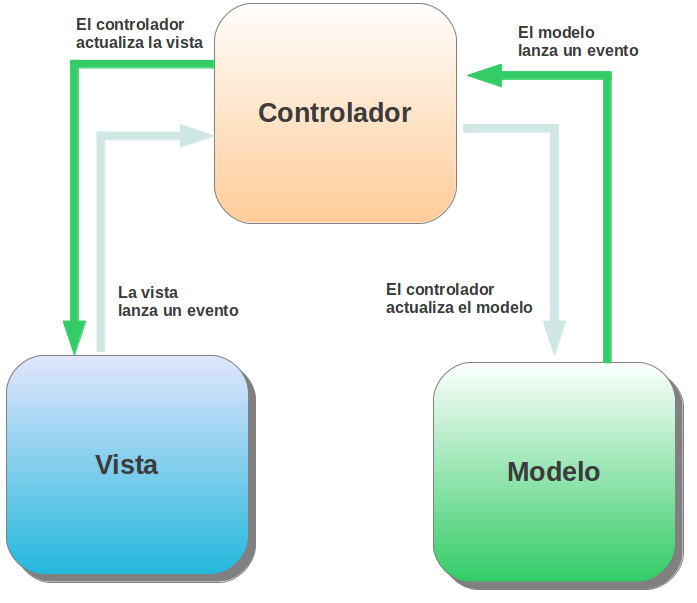
\includegraphics[width=300px, height=300px]{img/mvc}

\begin {itemize}


  	

\item {\bf Modelo}
	El modelo maneja el comportamiento y los datos del dominio de la aplicaci�n,
	responde a los pedidos de informacion sobre su estado (por lo general de la
	vista), y responde a las instrucciones para cambiar su estado (por lo general
	desde el controlador). Tambi�n deber�an ser capaces de soportar	m�ltiples presentaciones
	
	
\item {\bf Vista}
	Muestra la informacion del modelo al usuario. 
	
\item {\bf Controlador}
	Es el intermediario entre el modelo y la vista.
	Mapea acciones del usuario con acciones al modelo.
		
	
\end {itemize}

\subsection{Eventos}


\subsection{Binding}
El Binding permite conectar la propiedad de un objeto (modelo) con otra de
otro objeto(vista).\\

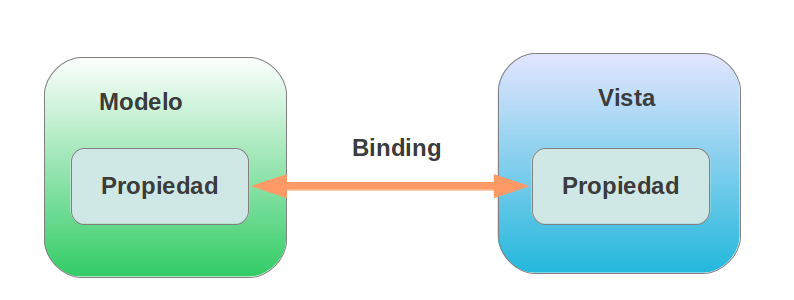
\includegraphics[width=300px]{img/binding}

Asociando estas dos propiedades, el flujo entre ambos puede asociarce en dos
modos.

\begin {itemize}

\item {\bf OneWay}
Con este tipo de binding el flujo de datos se realiza en una sola direcci�n. 

\item {\bf TwoWay}
En este tipo de asociaci�n el flujo se produce en ambas direcciones. Los cambios
realizados en el modelo se ven reflejados  en la vista y viceversa. (Este es el
tipo de binding que tenemos en el Arena)

\end {itemize}

\subsubsection{Ventajas}
Al tener vinvulados los datos entre la interfaz y el modelo

\subsubsection{DesVentajas}
Al no existir esa vinculacion, los datos que se tienen que pasar del modelo a la
interfaz y viceversa , hay que hacerlo a mano.


\subsubsection{Problemas sin binding}

\subsubsection{Problemas con Binding}
	
\section{Transacciones}	
	
	

El objetivo de este trabajo es proponer una soluci�n a estos dos problemas que
minimice el impacto en el c�digo de las clases del dominio de la aplicaci�n


